\section{Experiments}

Based on \cite{griffiths2012bottom}, we wanted to remove the learner's access to a performance measure so as to create an interaction similar to what we have in \cite{grizou2013robot}.

\subsection{Method}

%In this experiment, we investigate how adult can negotiate

The purpose of this experiment was to simulate a basic human-robot interaction and study how human adults would perform in such situation. Specifically, the learner does not have access to a measure of its performance; the teacher can only understand the intention of the learner thought its external, not explicitly communicative, behaviour; and the learner can only process information in a sequence of symbolic signals. To illustrate this scenario, we consider a construction task, were a teacher must explain to a learner what construction must be build with the blocks present on a table.


\subsubsection{Participants}

The 36 participants (31 M / 5 F), recruited among students and staff at INRIA Bordeaux Sud-Ouest, were divided into teachers and learners. They registered to be participants beforehand. The age range was between 20 and 35 and their average was 24 years.

\subsubsection{Stimuli}

The teacher and the student were in separate rooms and had only access to selected information displayed on a screen. For the purpose of the present study, we developed a simple computer interface. On the student side, a computer was displaying symbols associated to button-presses from the teacher. On the teacher side, a computer was displaying the blocks moved by the student recorded by a webcam on the student side. To send signals to the student the teacher had access to a box equipped with 10 buttons, see figure~\ref{fig:box}. Each button was randomly mapped to a symbols and screen position on the student side. We tried to use neutral symbols, see figure~\ref{fig:sign}.

There were 12 primary-coloured Mega Blocks$^{\textregistered}$ blocks of different size (see figure~\ref{fig:duplos}); 3 red two-pads, 2 red three-pads, 2 yellow four-pads, 2 blue three-pads, 2 green two-pads, and 1 green four-pads blocks. During preliminary tests, we found that leaving the teacher with a free choice for the aimed construction was unproductive. We therefore presented the teacher with 20 construction's pictures from which they should choose one, see figure~\ref{fig:constructions}. A construction does not necessary contain every blocks.

\begin{figure}[H]	
	\centering
	\begin{subfigure}[t]{0.32\columnwidth}
		\centering
		
\includegraphics[width=\columnwidth]{sign.png}
		\caption{Three examples of sign displayed on the learner screen}\label{fig:sign}		
	\end{subfigure}
	\begin{subfigure}[t]{0.32\columnwidth}
		\centering
		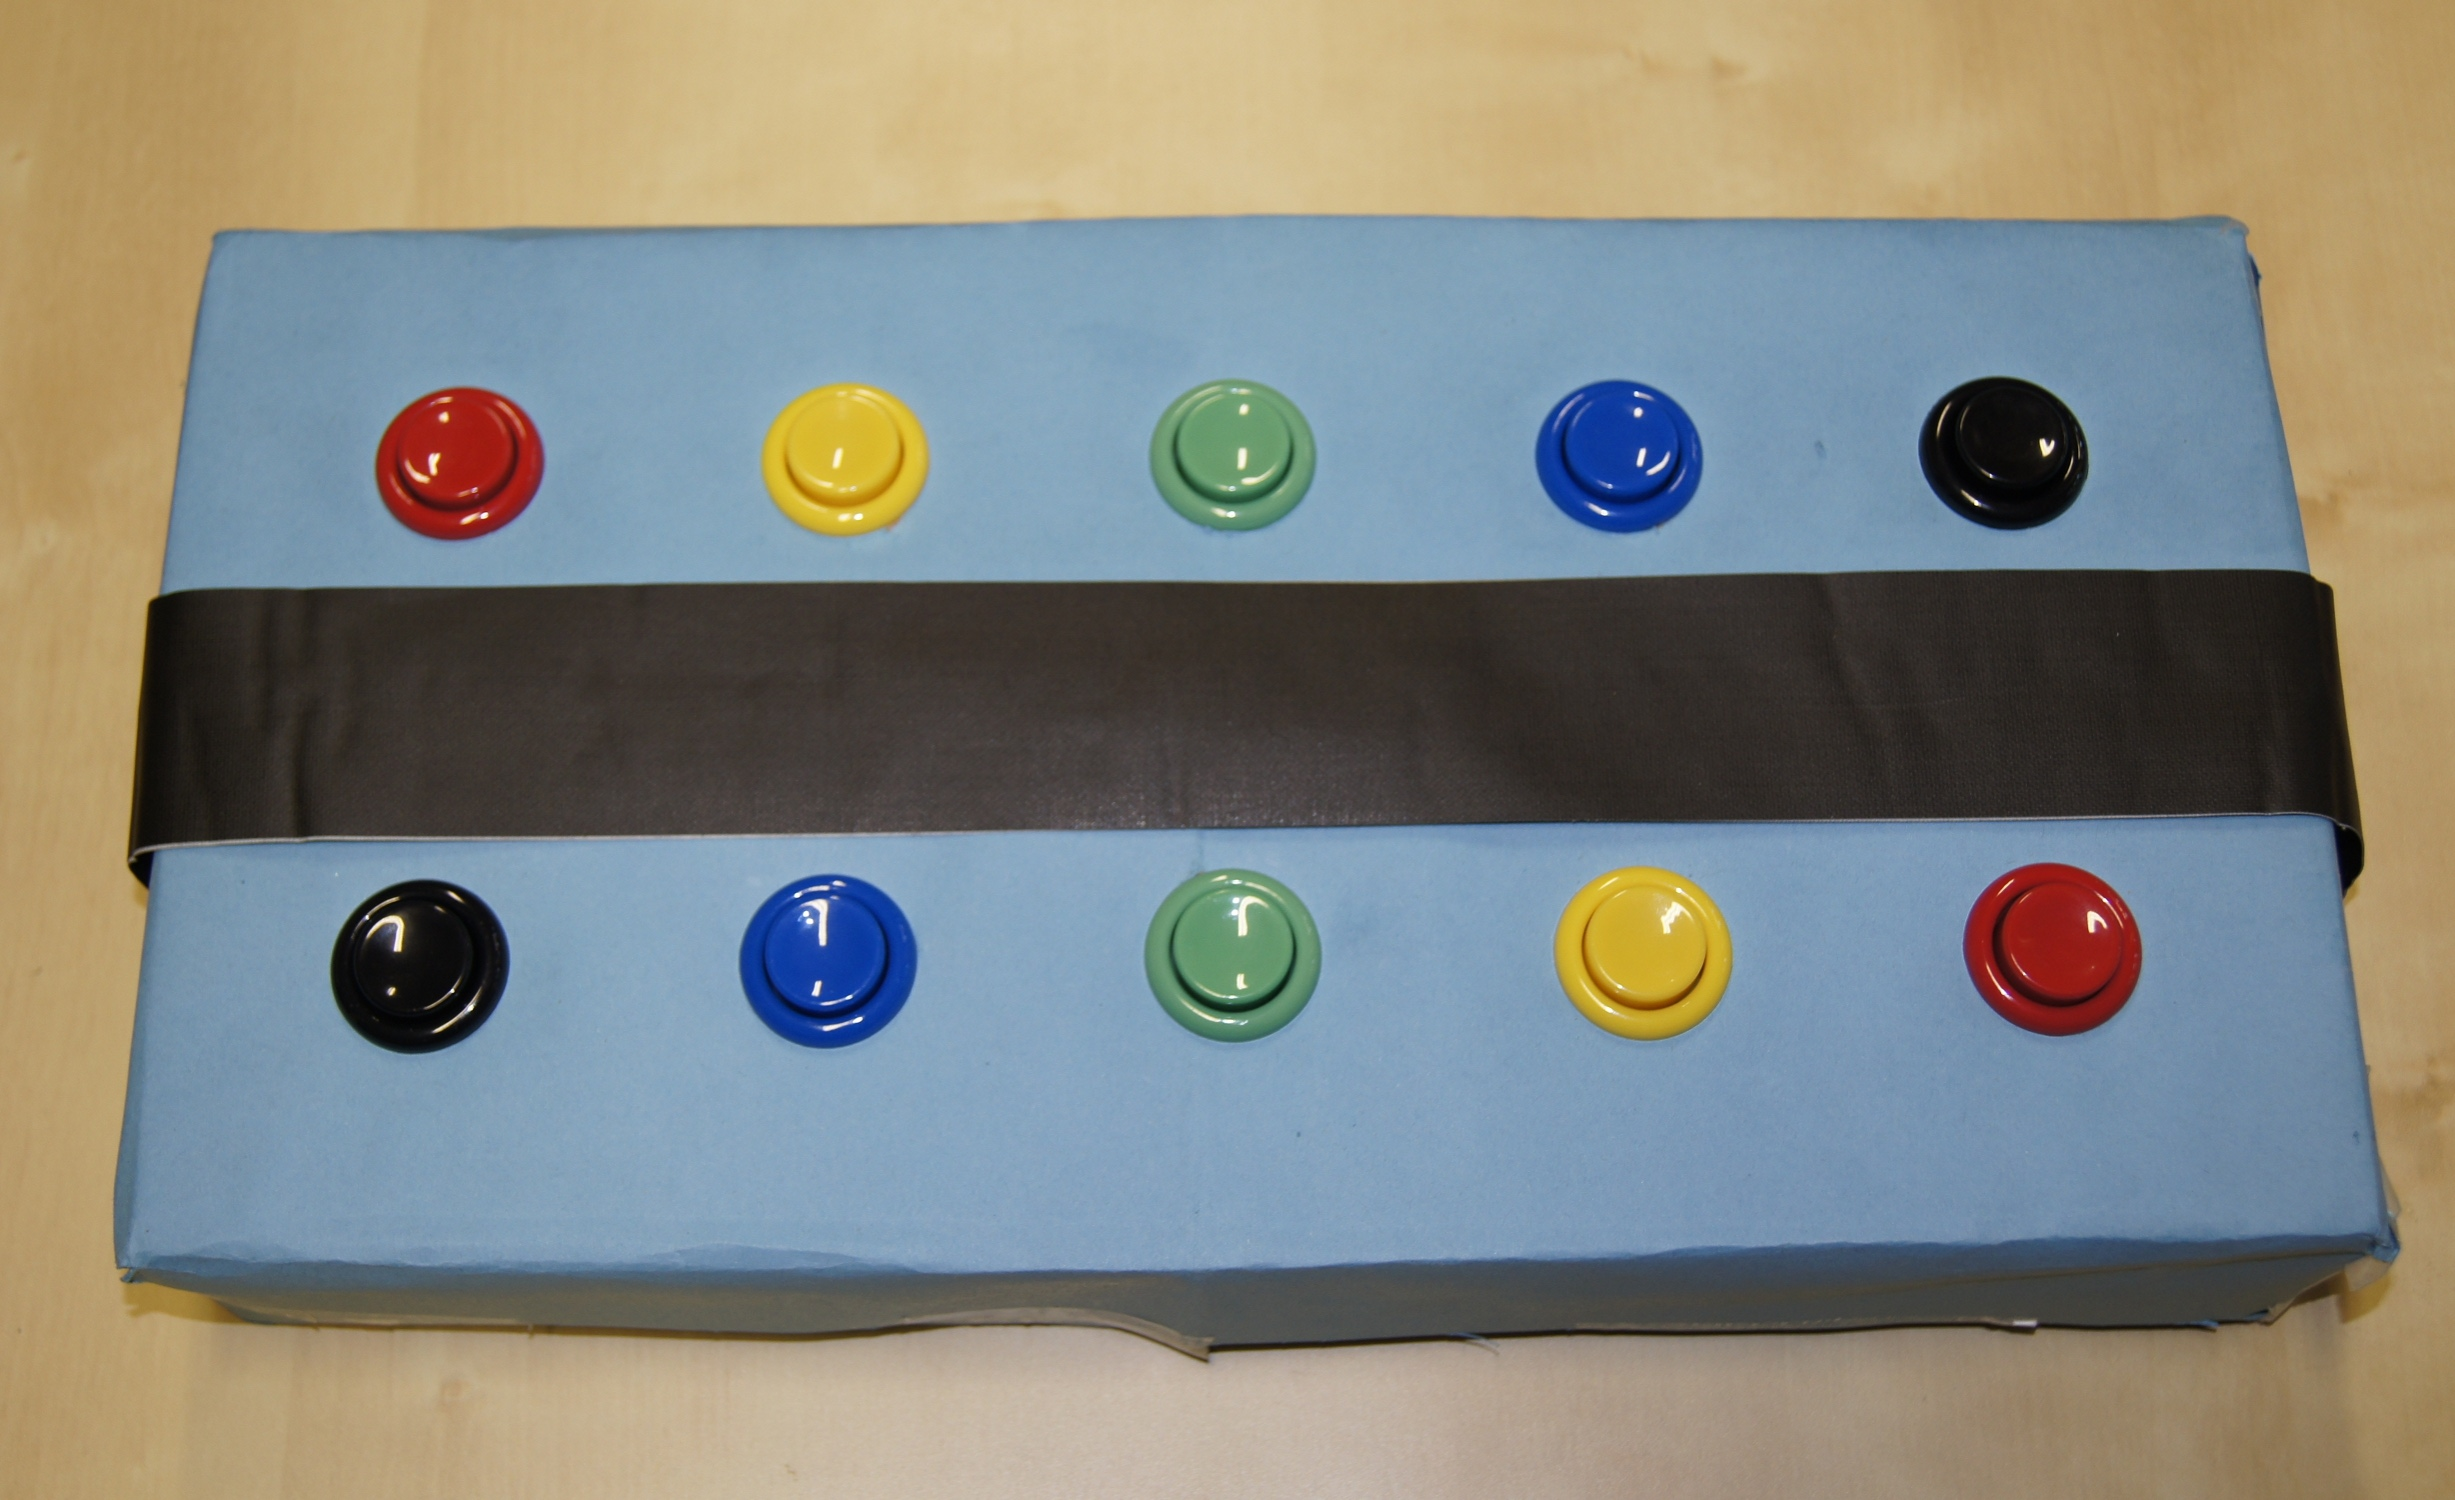
\includegraphics[width=\columnwidth]{box.jpg}
		\caption{The box and the button use as an interface for the teacher to communicate with the learner}\label{fig:box}
	\end{subfigure}
	\begin{subfigure}[t]{0.32\columnwidth}
		\centering
		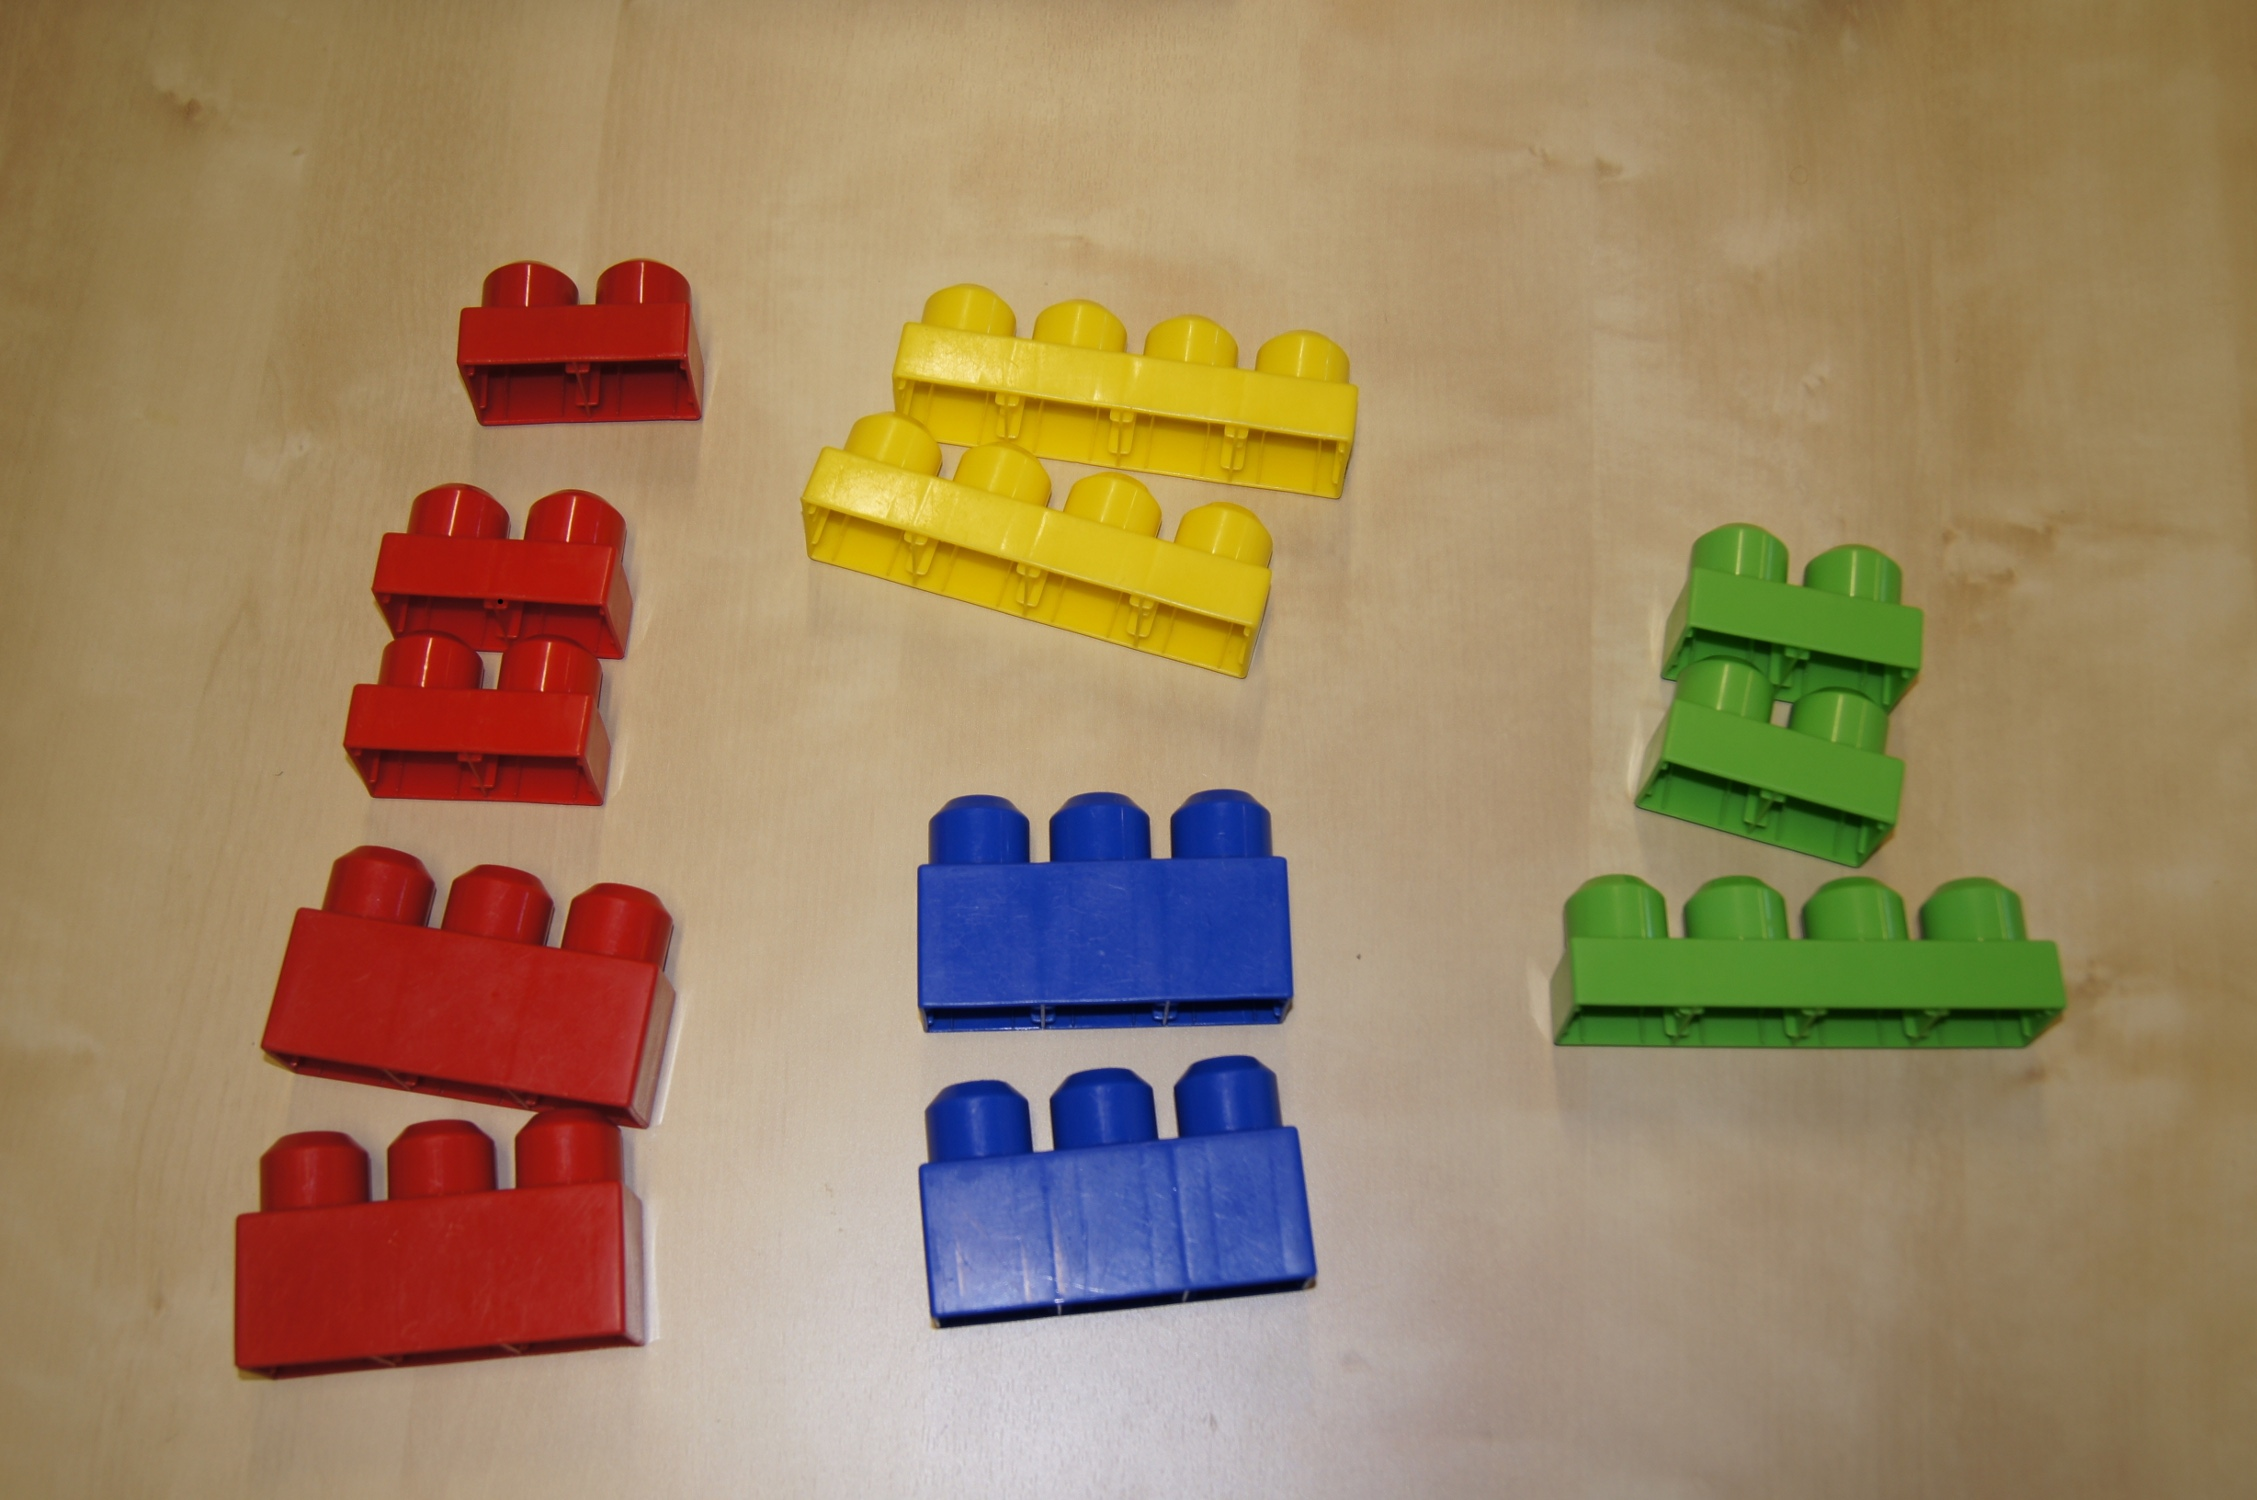
\includegraphics[width=\columnwidth]{duplos.jpg}
		\caption{The blocks used in the construction task}\label{fig:duplos}
	\end{subfigure}
	\begin{subfigure}[b]{\columnwidth}
		\centering
		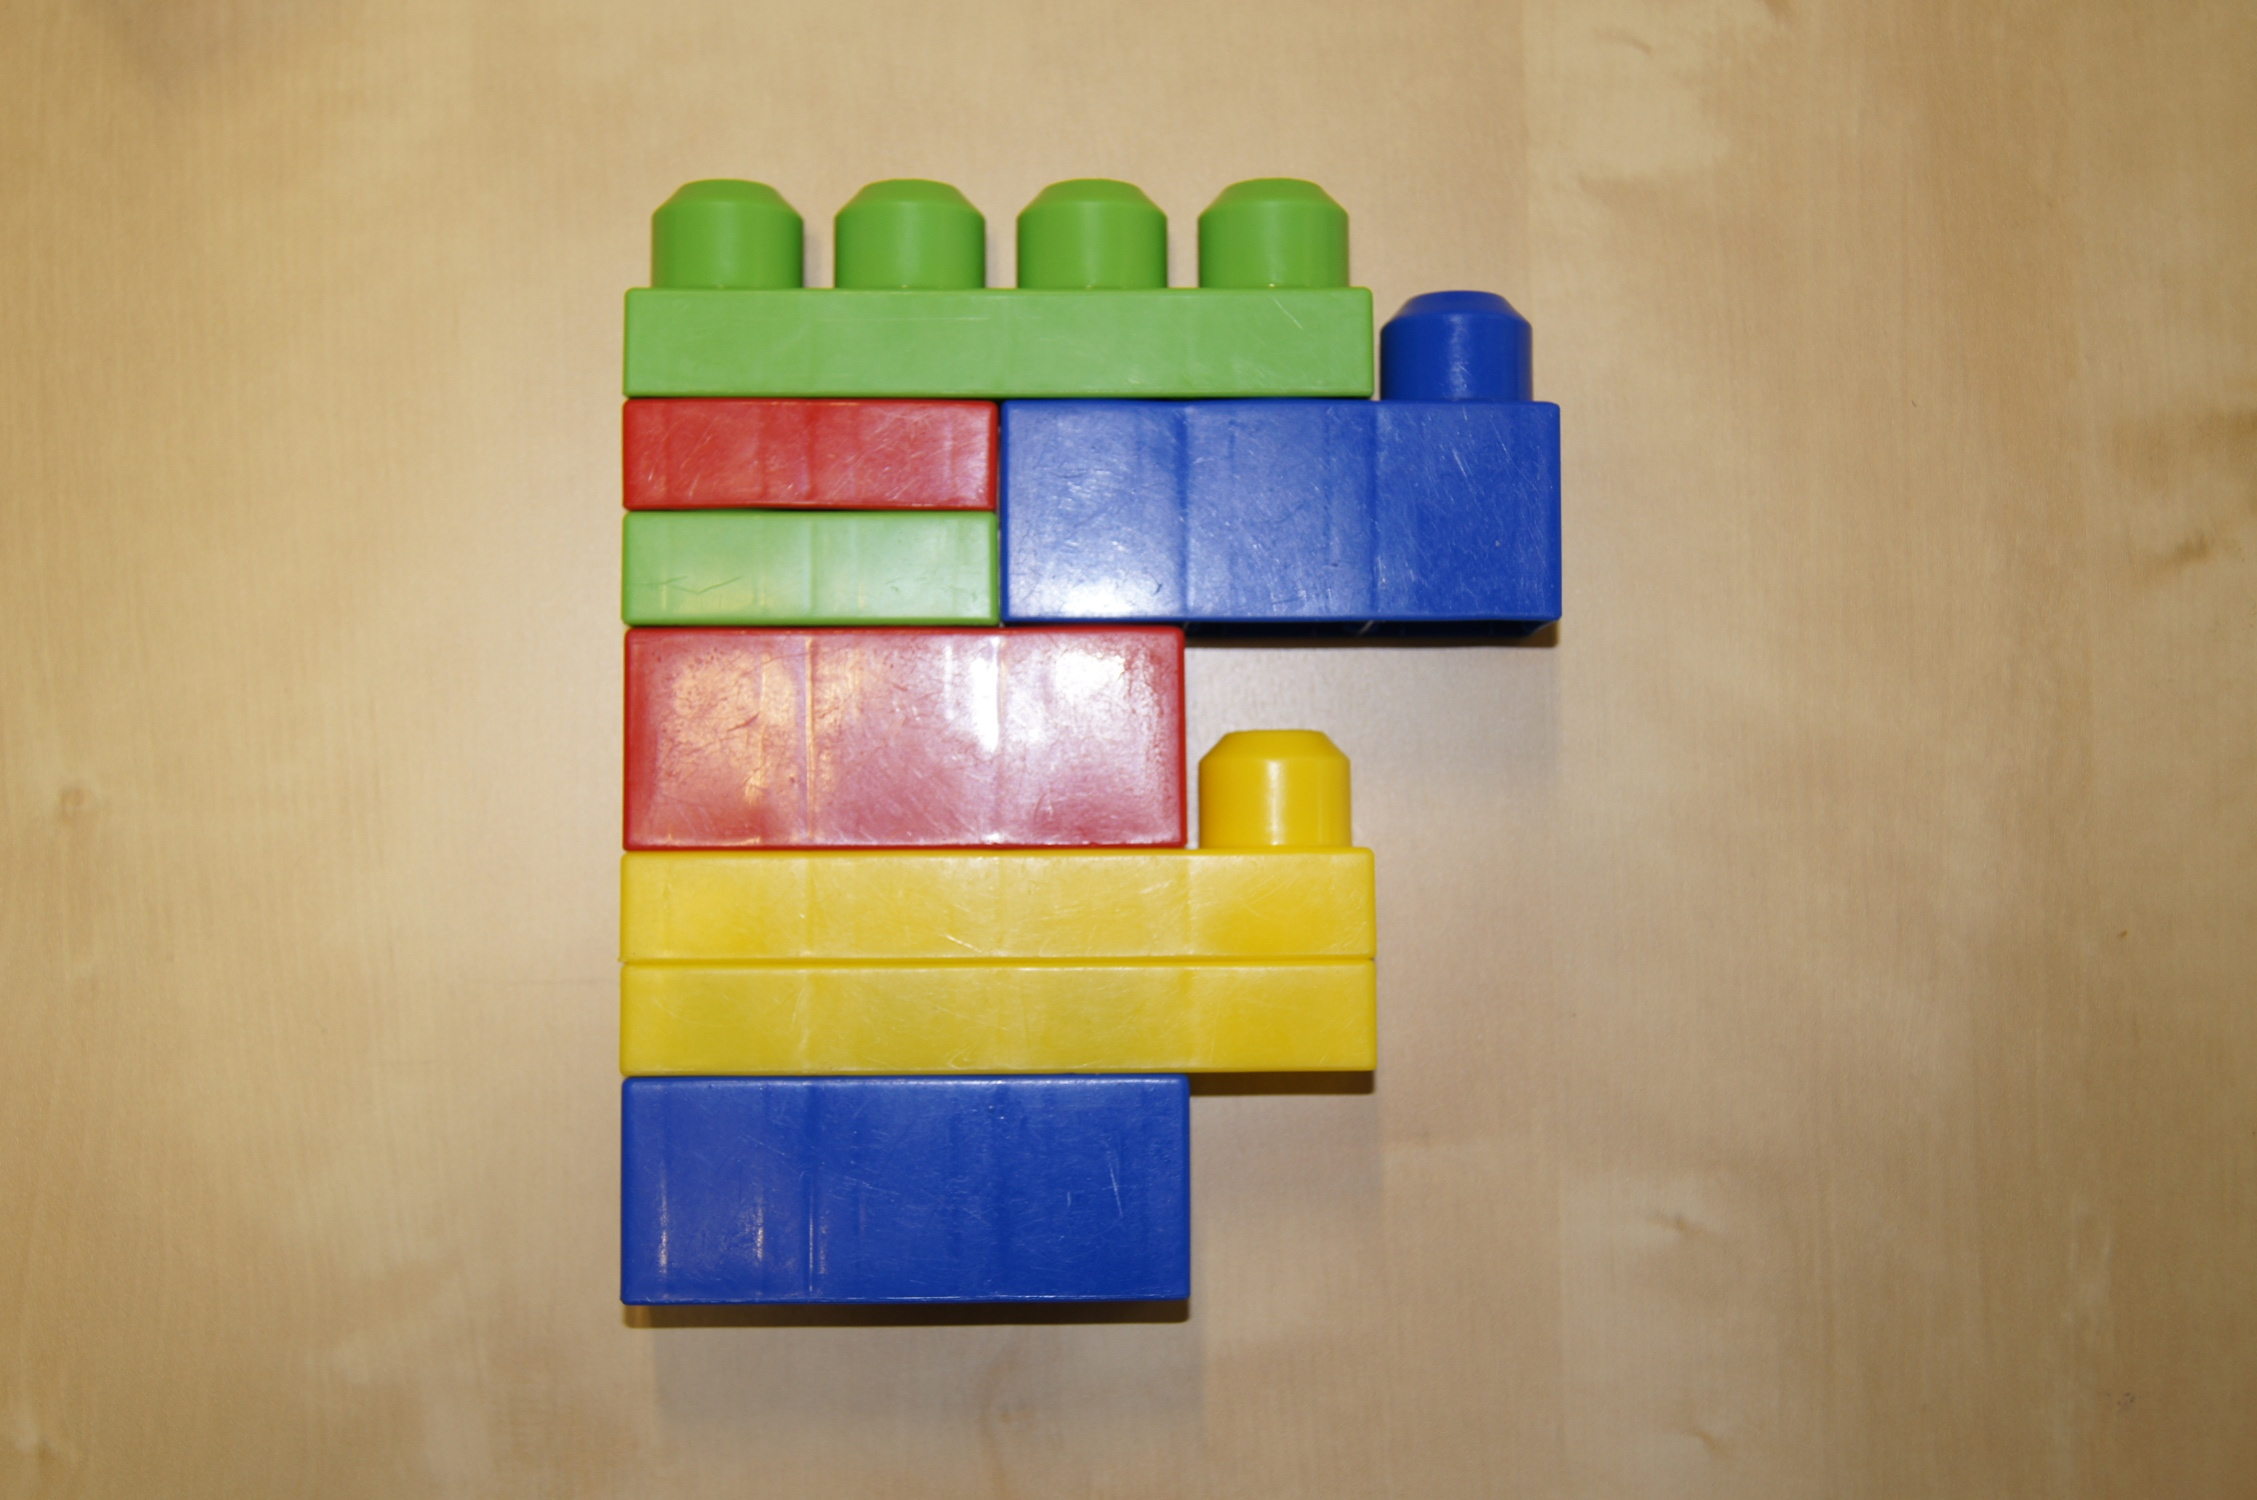
\includegraphics[width=0.24\columnwidth]{foo/_DSC4111.JPG}
		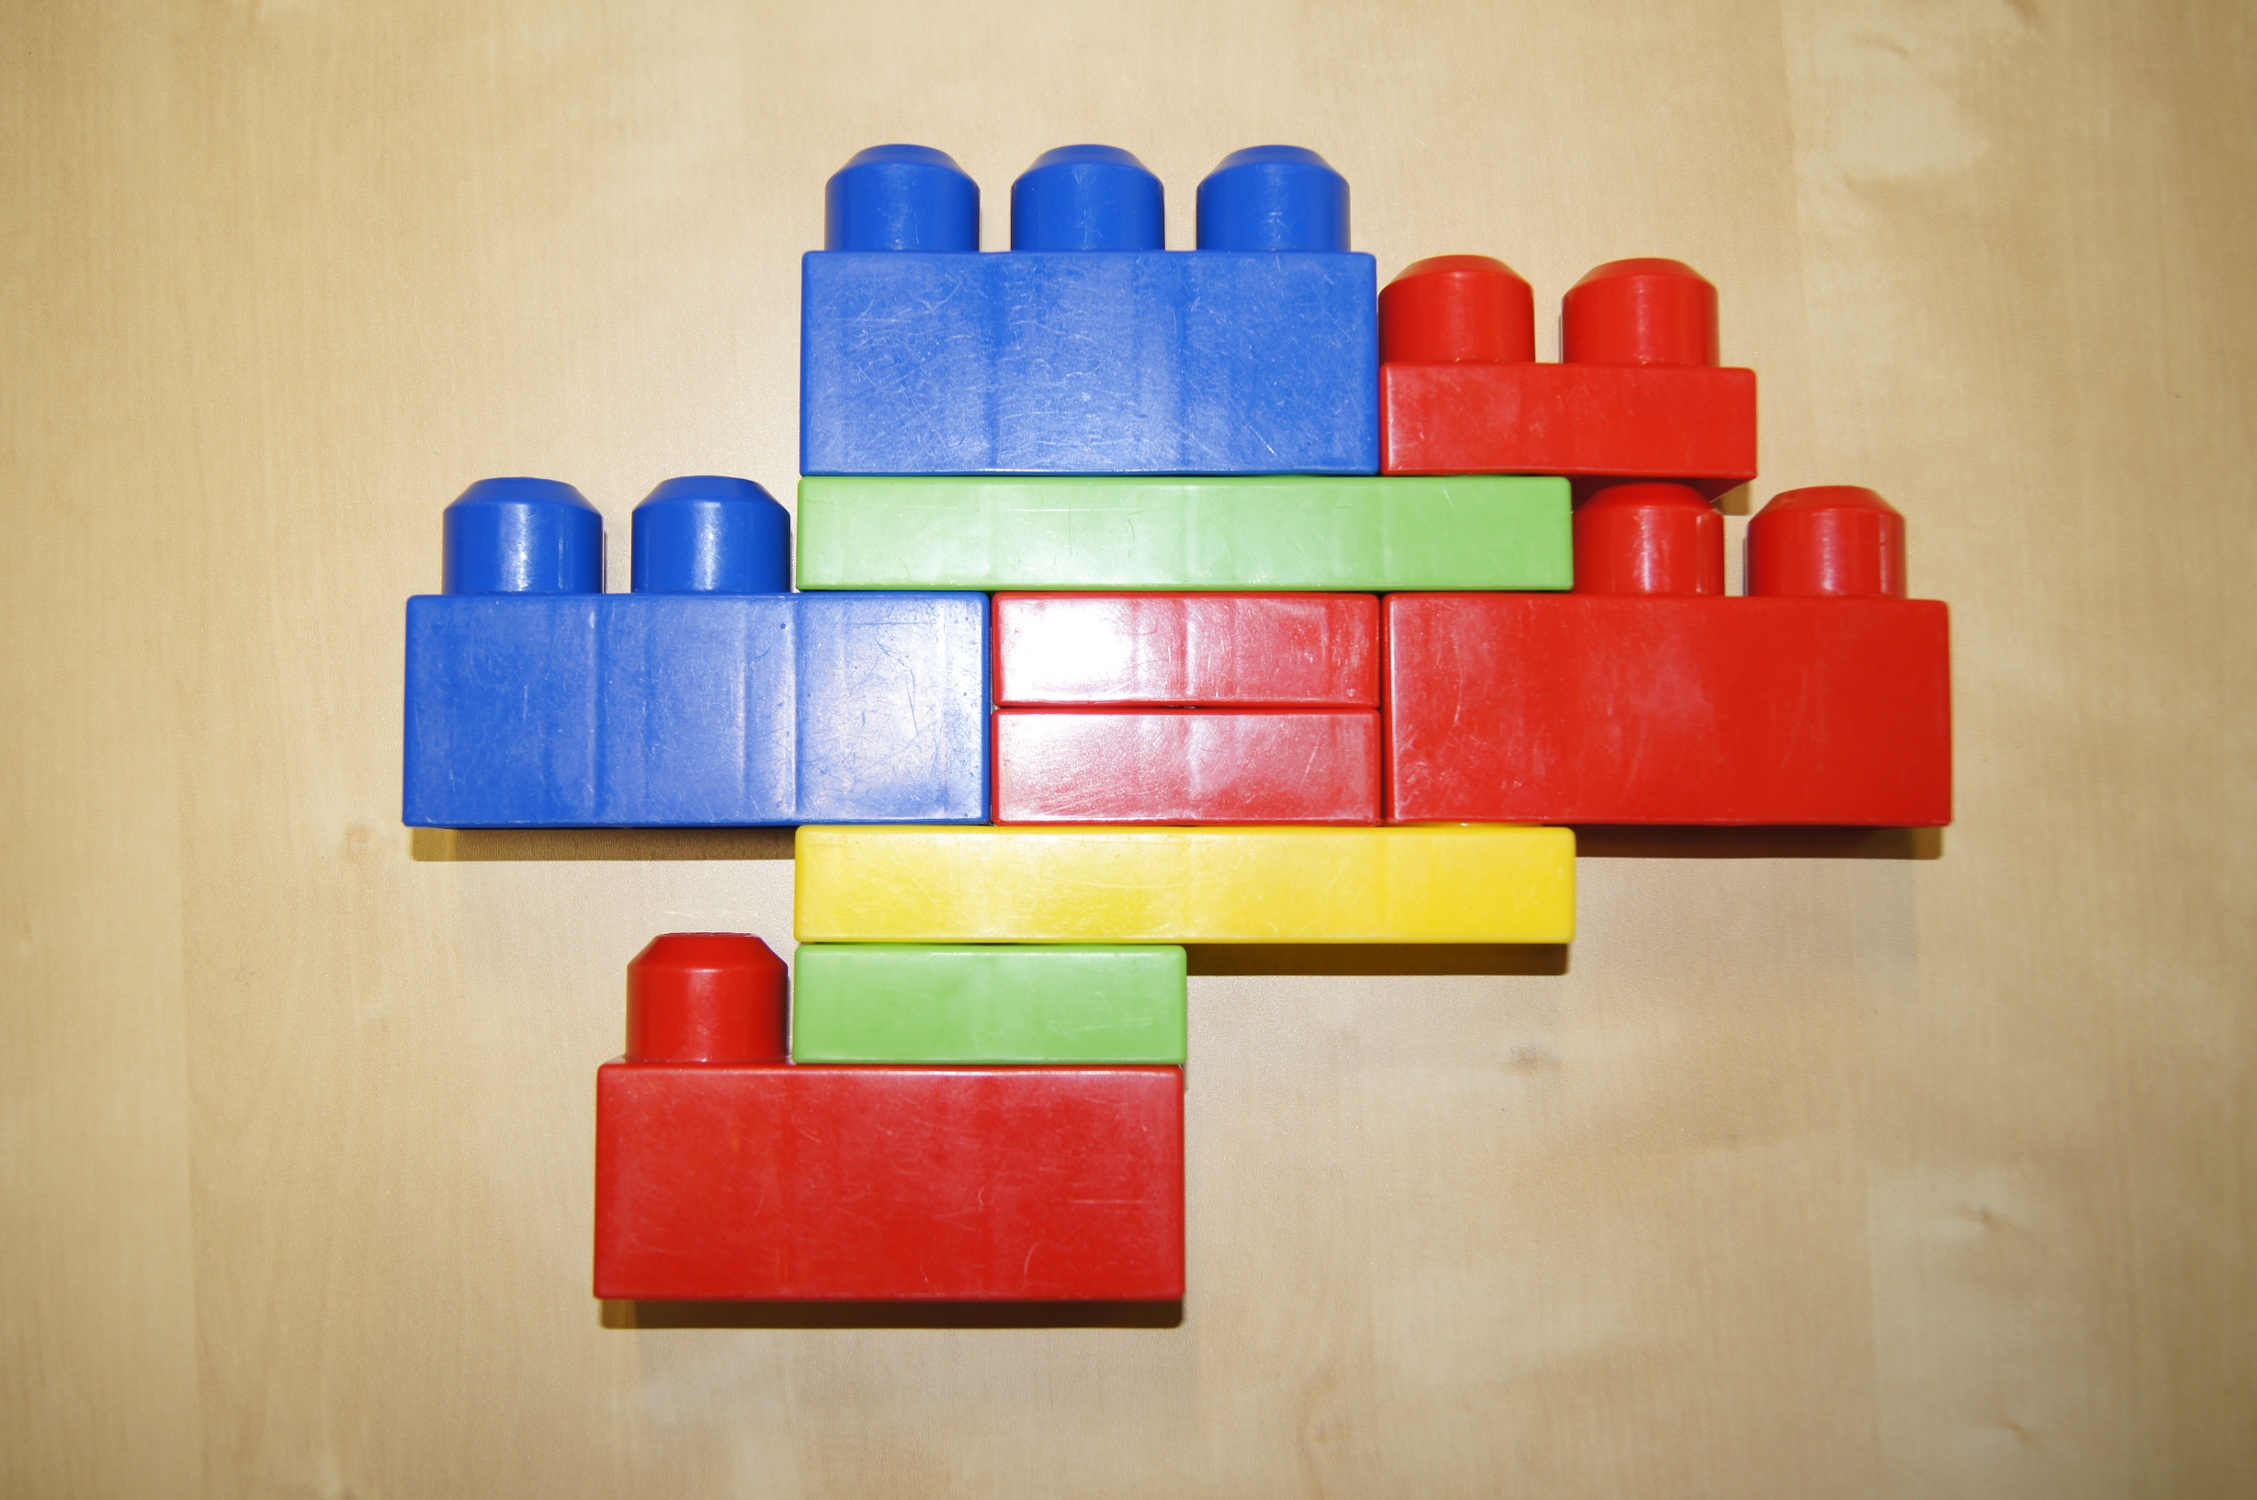
\includegraphics[width=0.24\columnwidth]{foo/_DSC4119.JPG}
		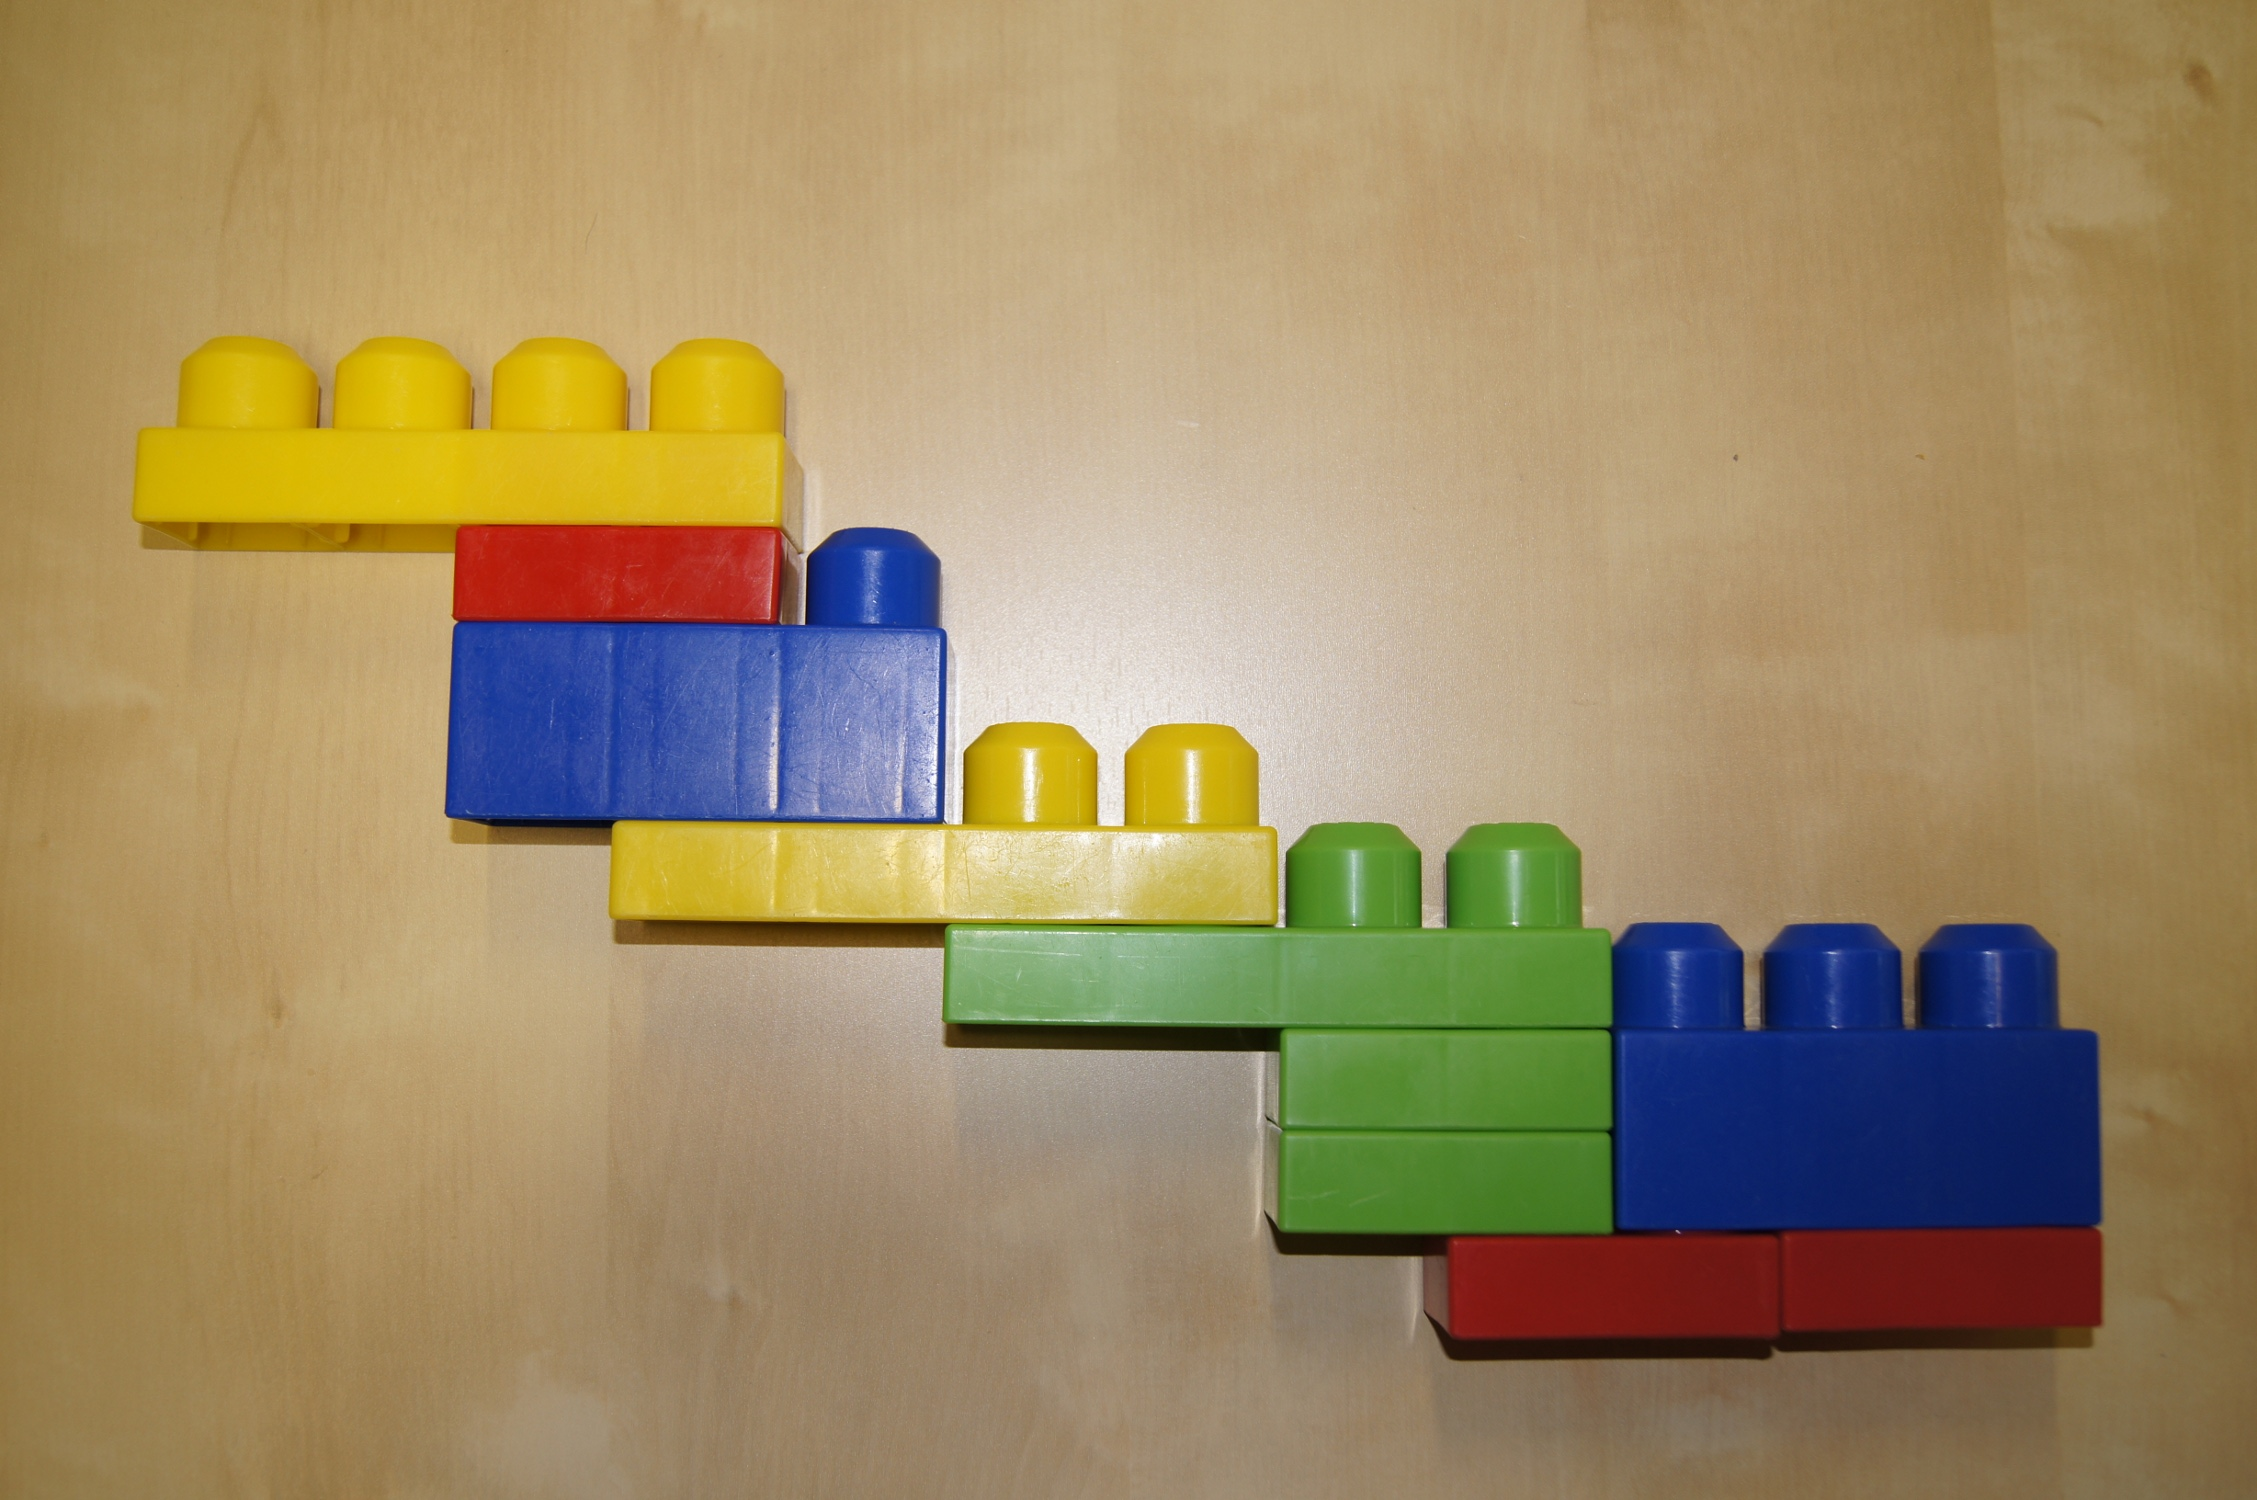
\includegraphics[width=0.24\columnwidth]{foo/_DSC4115.JPG}
		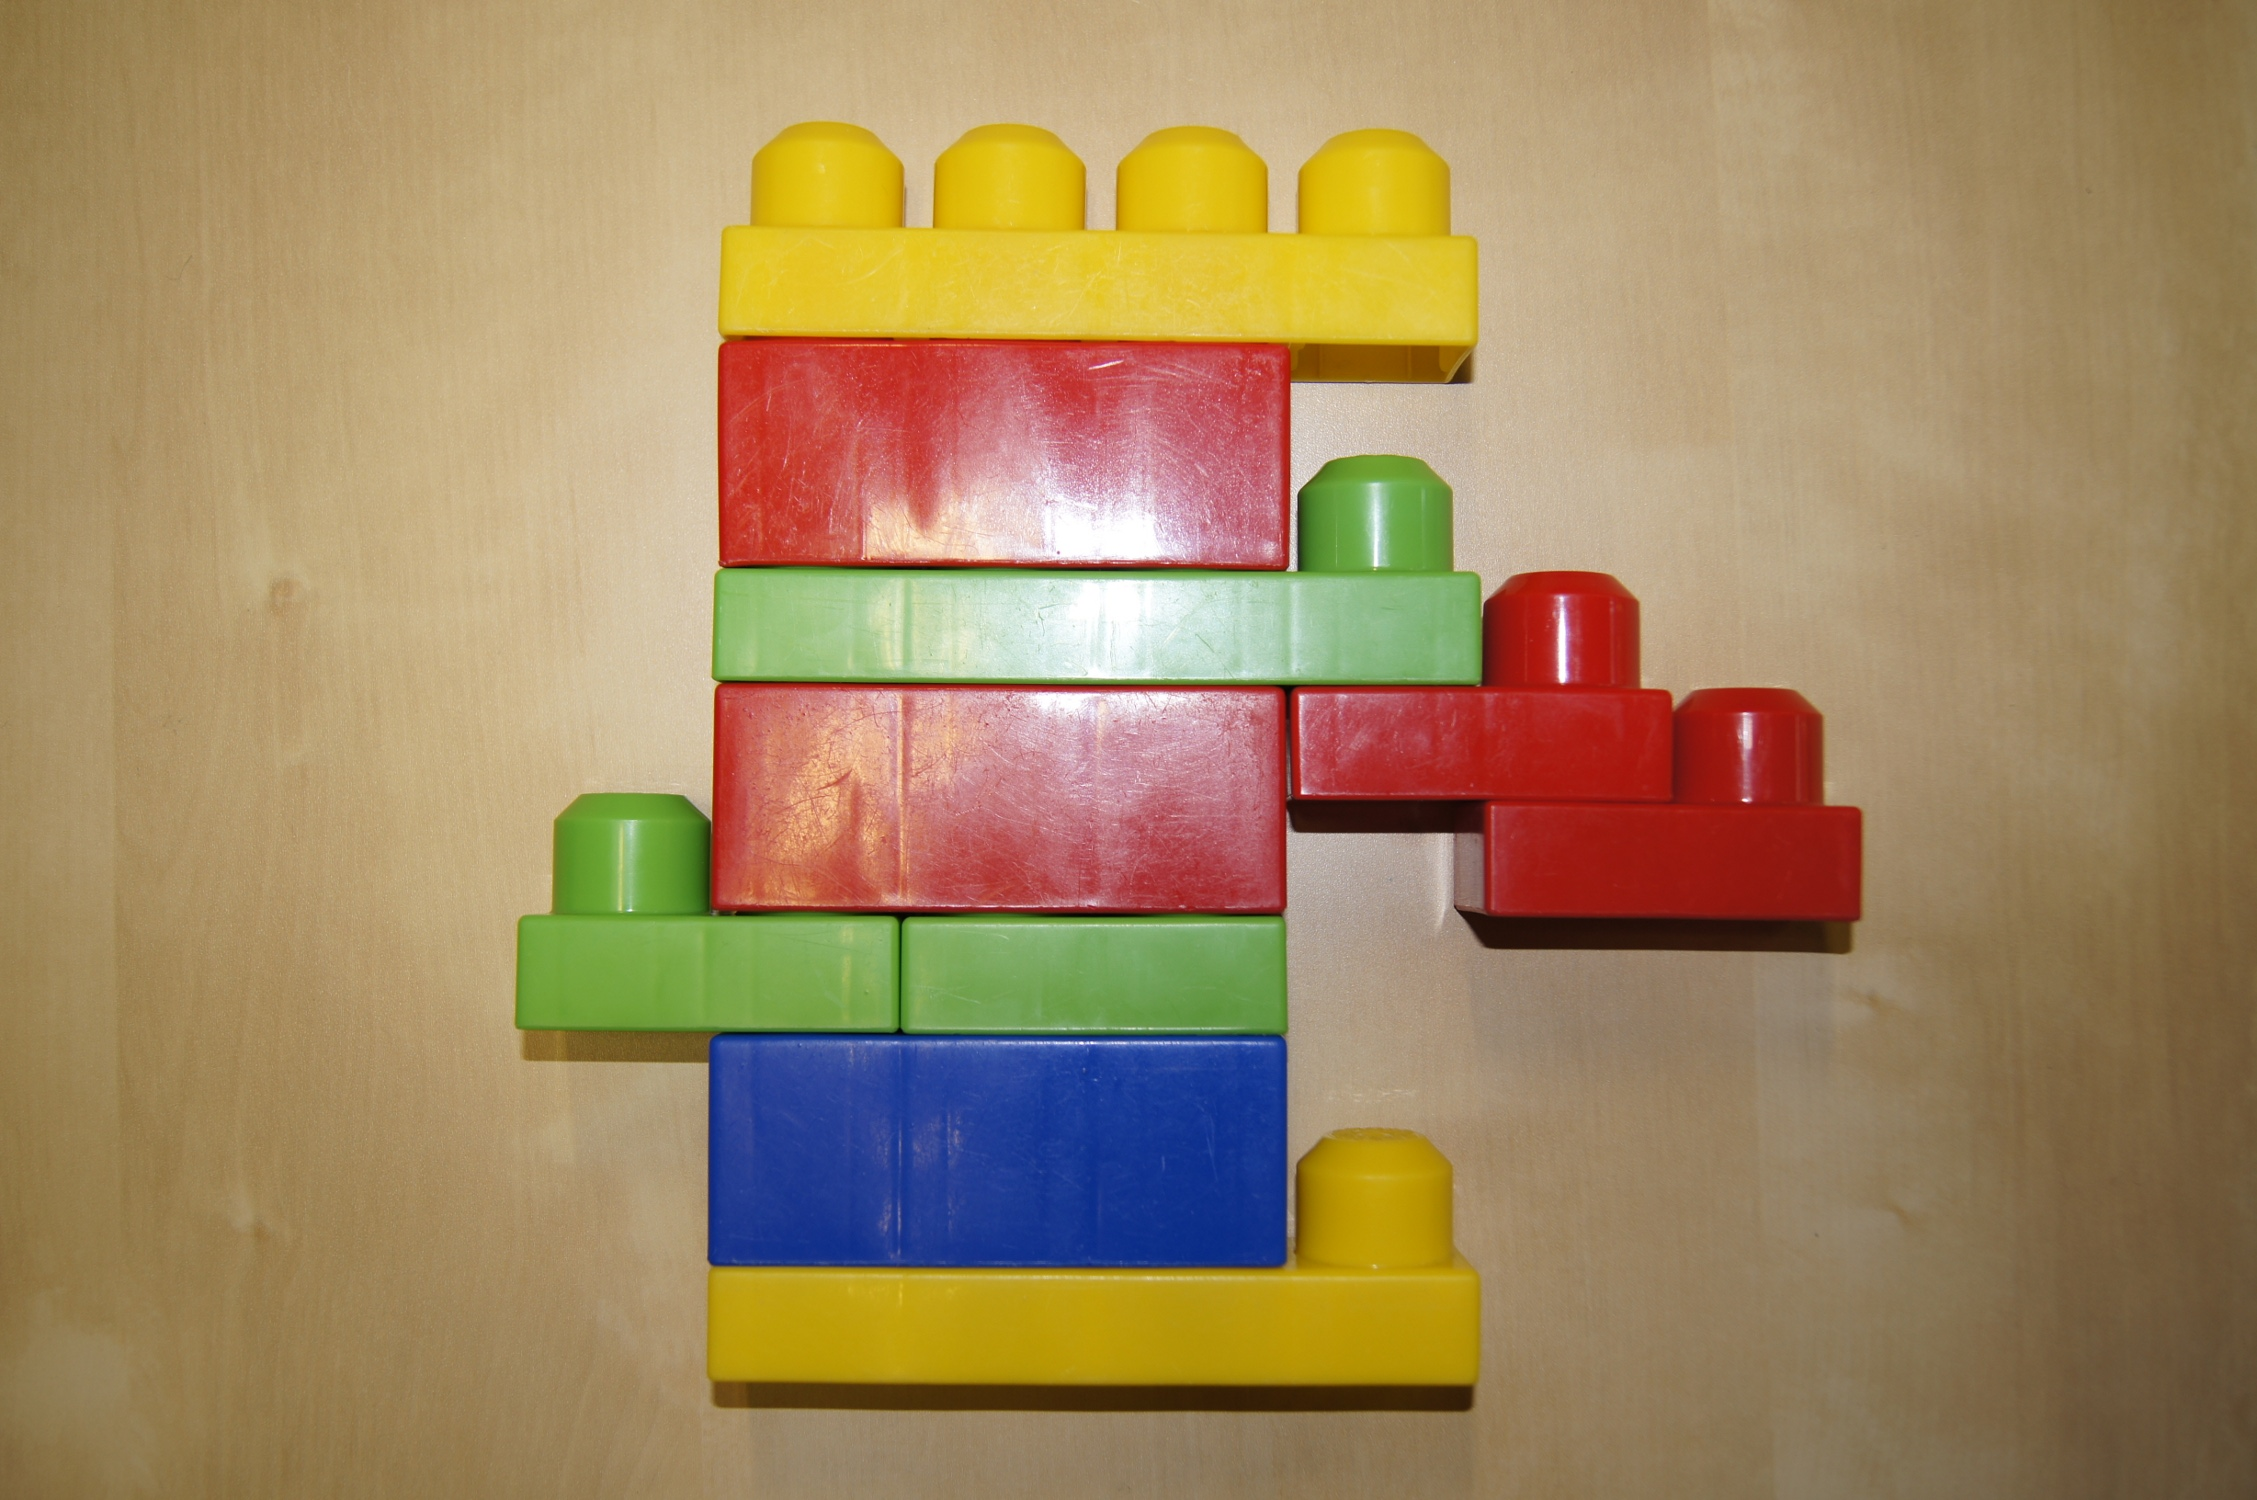
\includegraphics[width=0.24\columnwidth]{foo/_DSC4118.JPG}
		\caption{Four examples of construction presented to the teacher}\label{fig:constructions}
    \end{subfigure}
    \caption{}\label{fig:setup}
\end{figure}

\subsubsection{Procedure}

The study was conducted in two separate rooms. Teacher and learner never talked about the experiment before and were explained the task only once isolated in their respective rooms. After explaining the task to each participant, the experiment starts. We reduced as much as possible the pause between explanation and experiment's start, so as they could not try to elaborate a teaching/learning strategy before starting. 

The teacher saw the building area from the student side. The student saw symbols displaying on a screen as an indication of button pressed by the teacher. The learner manipulate the blocks and try to build the construction the teacher has in mind. The teacher presses the button so as to guide the student in building the construction it has in mind. A construction is made of any number of blocks at least linked by one pad. The manipulation of the button is the only way for the teacher to communicate with the learner. The spacial organization of button is different than the spacial organization of displayed symbol on the learner side. The teacher is aware that the mapping is different but not of the actual mapping. This way the teacher can not give direct spatial indication. The observation of the screen was the only way for the student to receive instructions from the teacher. The experiment stopped when the student decided the construction he had build was correct.

\subsection{Results}

For the experiment we did this summer, we recorded only the timing in button presses and the video the teacher was seeing. In addition, we took notes on both side (teacher/learner) on what participants where thinking, what buttons or displayed symbols meant, and the rough evolution of such meaning (not timed). We ran a total of 18 experiments, 14 were successful and 4 failed. The average duration of one experiment was 18 minutes with a minimum of 7 minutes and a maximum of 45 minutes.

The first analysis concerns types of instructions. When analysing the different types of instructions the participants were using, we created 9 categories.
\begin{enumerate}
    \item \textbf{Positive Feedback}
    \item \textbf{Negative Feedback}
    \item \textbf{End:} A signal identifying that the construction is finished 
    \item \textbf{Reset}
    \item \textbf{Guidance:} A signal informing what to do. It includes \emph{change, invert, revert, new block, continue, stack} 
    \item \textbf{Colour:} A signal referring to colour of a block. It includes \emph{yellow, blue, red, green}
    \item \textbf{Size:} A signal referring to size of a block. It includes \emph{small, medium, big}
    \item \textbf{Location:} A signal referring to location of a block. It includes \emph{under, above, left, right}
    \item \textbf{Group:} A signal referring to group of block. It includes \emph{in, out, group\_X}
\end{enumerate}

For each experiment, we then identified if the teacher or the learner consider each type of instruction. The results are shown in figure~\ref{fig:types_of_feedback}. We note that for every experiment the positive and negative feedback instruction were considered. In addition, the \emph{End} instructions is often considered while more concrete instruction such as \emph{Guidance, Colour, Size, or Location} were not much considered, especially by the student.

\begin{figure}[H]
	\begin{center}
   		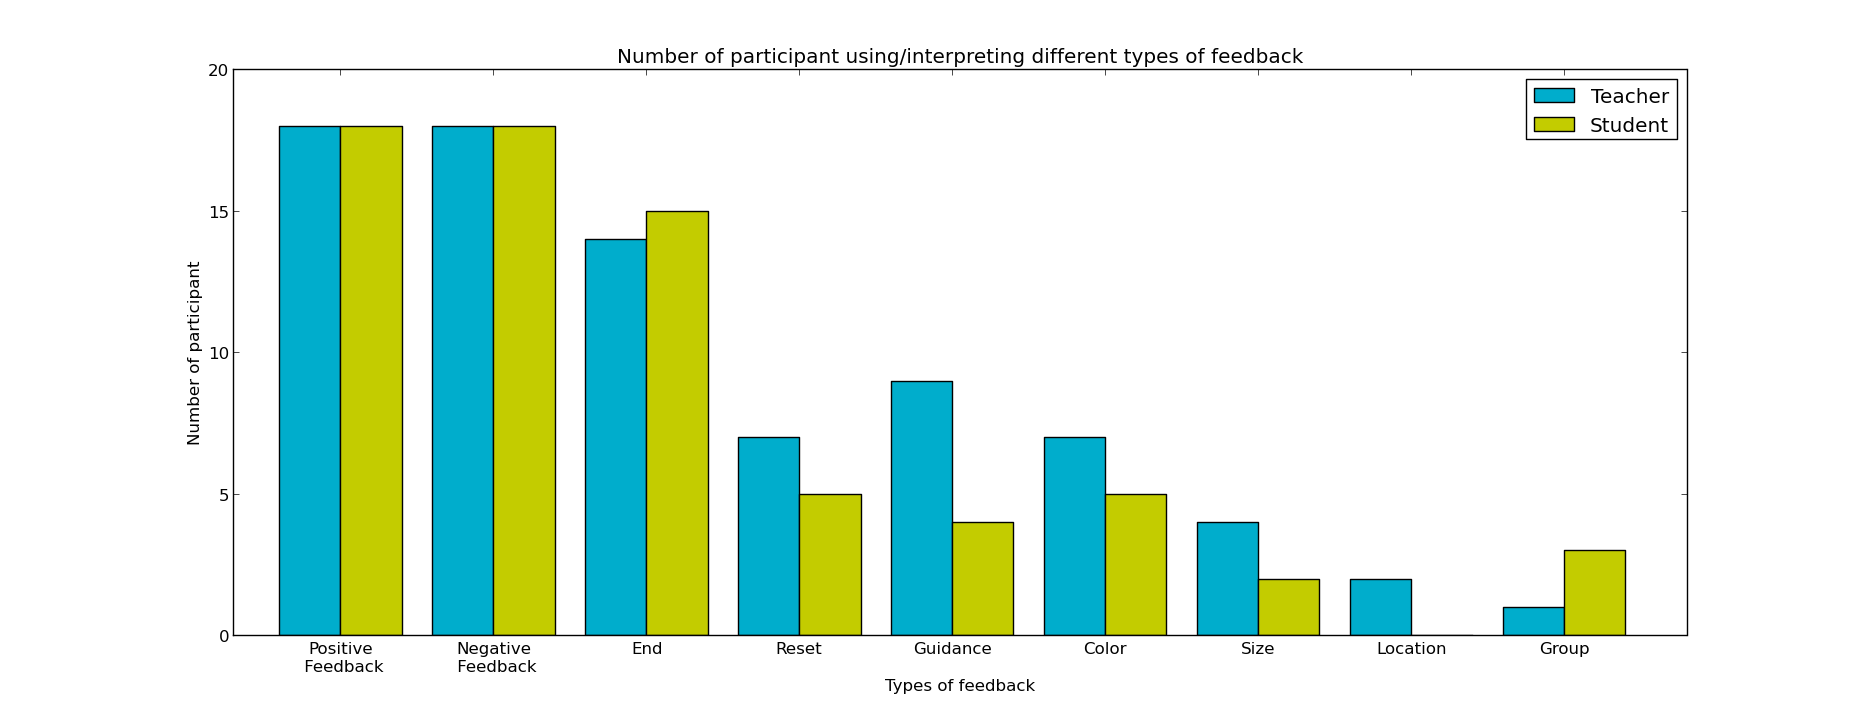
\includegraphics[width=\columnwidth]{types_of_feedback.png}
   		\caption{Number of participants that used (teacher) or interpreted (student) channels as conveying different types of instructions. All participants considered positive and negative feedback types of instruction.}
    \label{fig:types_of_feedback}
   	\end{center}
\end{figure}

From this results, it would be interesting to know to which extend the teacher and the learner understand each others. To do so, we compare the associated meaning of each button (or specific button pattern, e.g.\ all buttons pressed at the same time) at the end of the experiment for both teacher and learner. We can then count the number of button understood, misinterpreted, or ignored by the student. We can then average the results for successful and failed experiments, see figure~\ref{fig:types_of_understanding}.
We can note that for successful experiments, the average number of signal understood is 3.5 which mostly correspond to positive feedback, negative feedback, end, and occasionally reset when needed. Interestingly for failed experiments, this number drops to 1.2, with a larger amount of signals misinterpreted and ignored.

\begin{figure}[H]
	\begin{center}
   		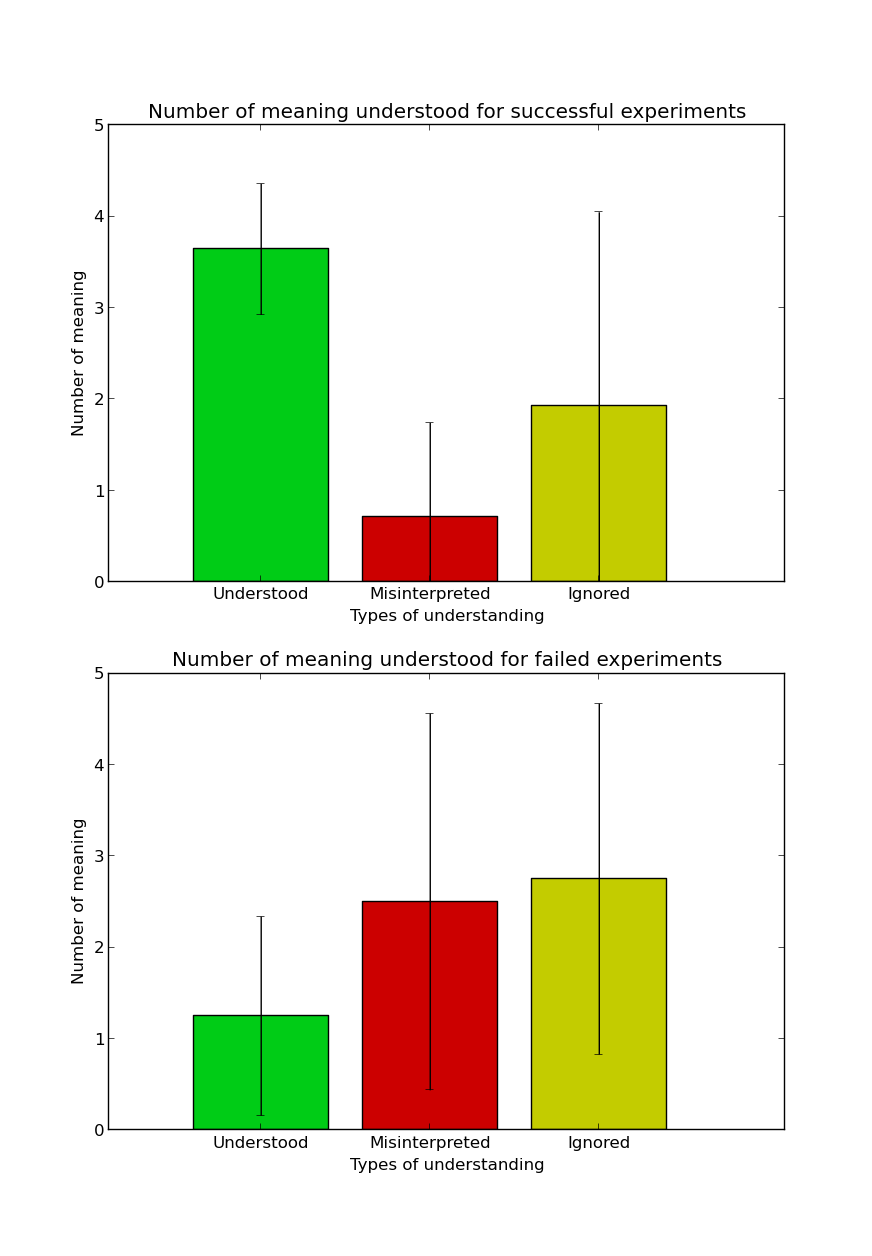
\includegraphics[width=0.4\columnwidth, trim=0cm 16cm 0cm 1.85cm, clip=true]{types_of_understanding.png}
   		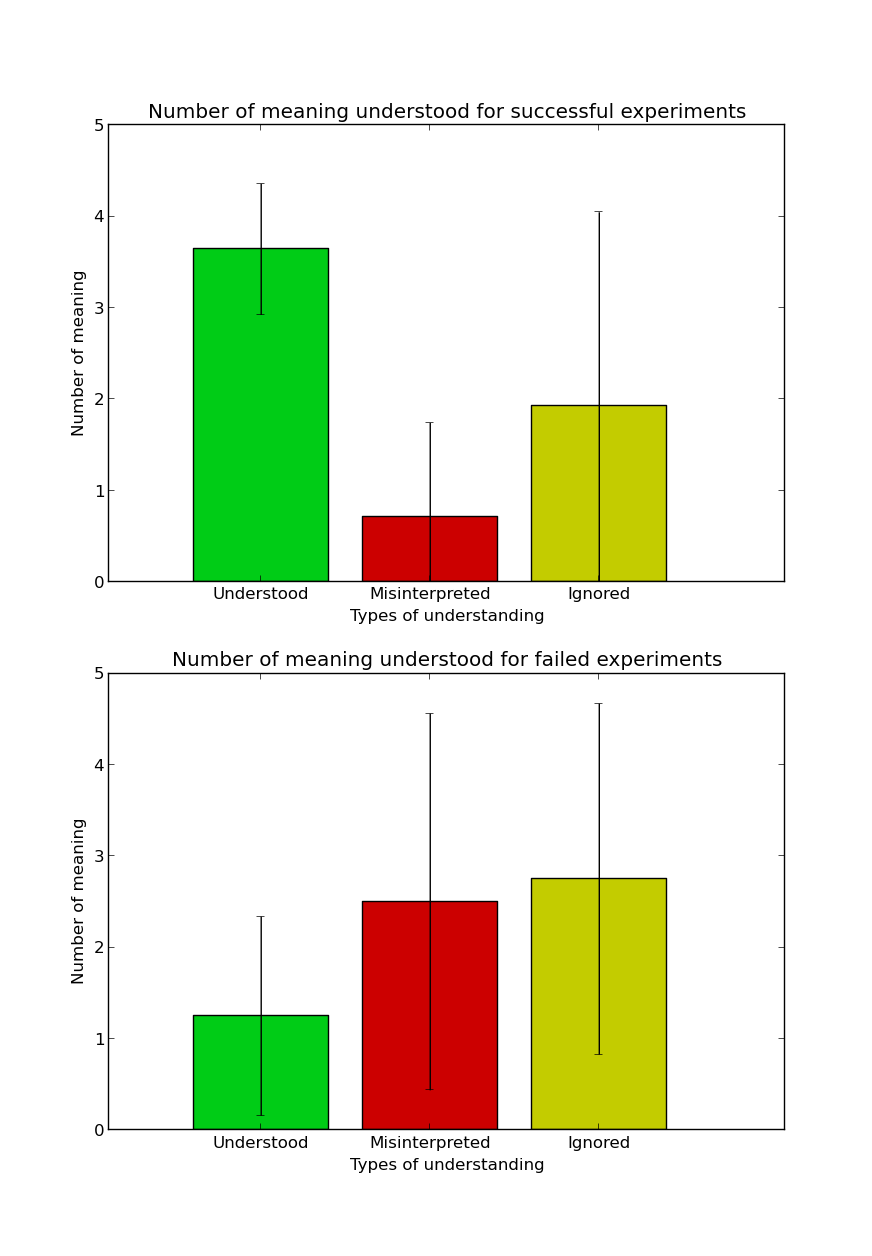
\includegraphics[width=0.4\columnwidth, trim=0cm 1.85cm 0cm 16.5cm, clip=true]{types_of_understanding.png}
   		\caption{Distribution of instruction channels that were understood, misinterpreted, and ignored by the learners. Data average across all learners for successful (left) and failed (right) experiments.}
    \label{fig:types_of_understanding}
   	\end{center}
\end{figure}

During the experiment, we noticed interesting properties on the feedback channels: some participants were inverting the meaning of such channel before, most of the time, detecting this misunderstanding and switching the meaning of button from positive to negative or the reverse. In few cases, it was the teacher that realized the learner were misinterpreting the signals but in most cases it was the learner that had to reinterpret the signals, often after a \emph{reset} instruction from the teacher. The data we collected are not enough detailed for this fine analysis but we are able to count the number of feedback interpretation switch per experiment, not their reason. This is shown in figure~\ref{fig:feedback_switch_enhanced}.

\begin{figure}[H]
	\begin{center}
   		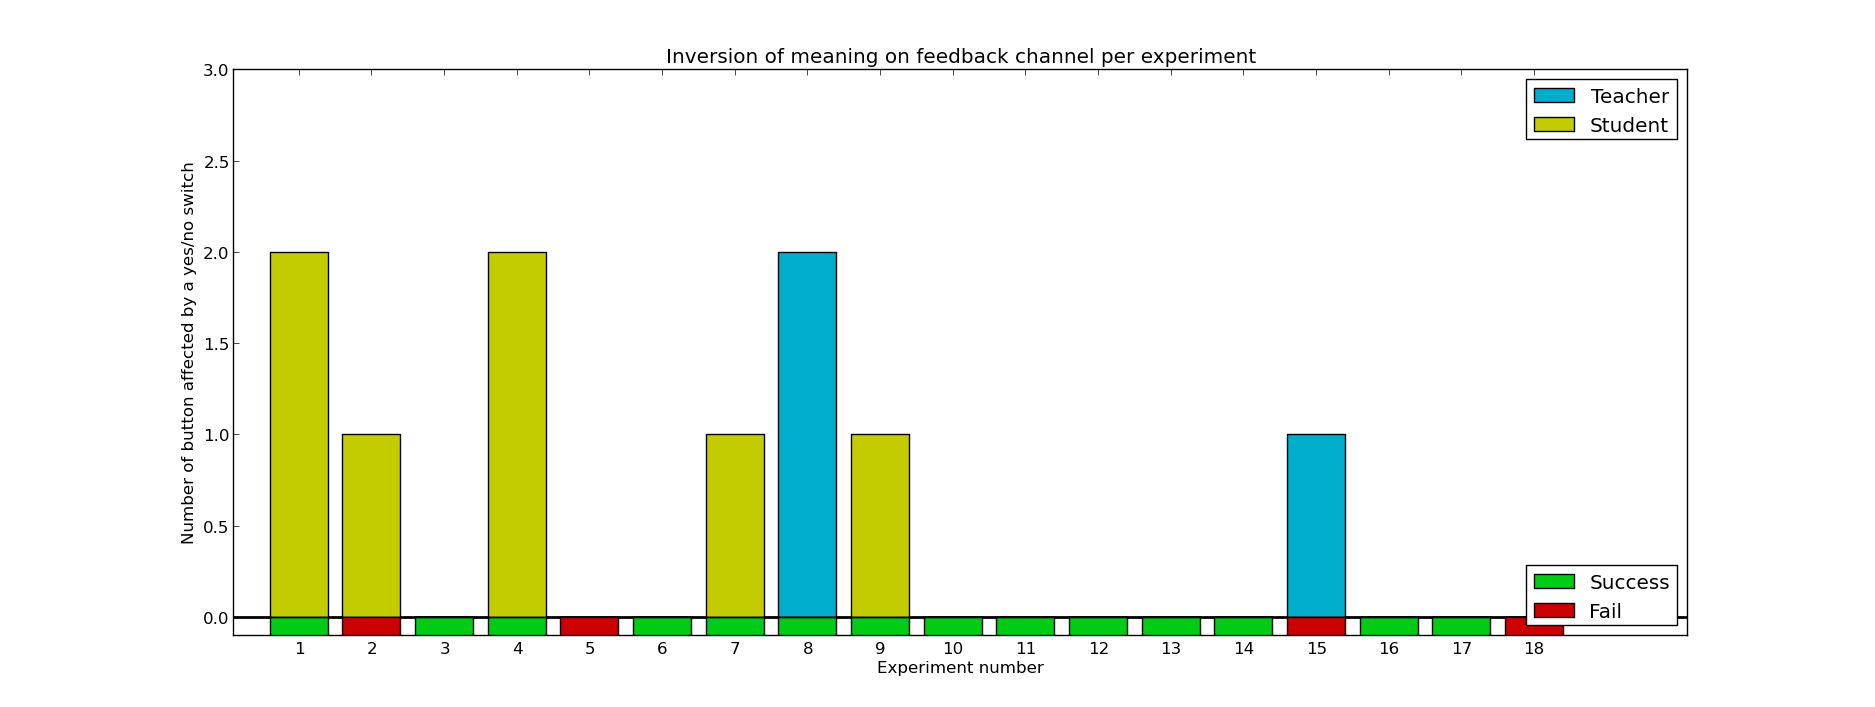
\includegraphics[width=\columnwidth]{feedback_switch_enhanced.png}
   		\caption{Number of channel whose meaning switch between positive and negative feedback during the experiment for the teacher and the student. In blue, cases when the teacher decides to change the meaning of a button from one feedback to the other. In yellow, cases when the student changed its interpretation of one button.The bottom coloured bar indicates if the experiment was successful or not. In 5 out of 14 successful experiments the teachers or the learners changed their use/interpretation of button between positive and negative feedback. A value of two indicate that student inverted the meaning of feedback channel, i.e.\ believing positive was negative and reversely, before either the teacher or the student fixed the misunderstanding.}
    \label{fig:feedback_switch_enhanced}
   	\end{center}
\end{figure}

An other interesting property is the context dependant meaning of some specific button presses patterns. For example, in several cases the teacher was pressing all buttons to signify a salient event. This event was either perceive as a \emph{Reset} instruction if the student felt lost or a \emph{End} instruction is the student felt confident about it understanding of the previous interaction sequences. This is illustrated in figure~\ref{fig:timeline}, where at $t=200 s$ the teacher presses all button to signify a \emph{Reset}. Indeed it seems he already tried several techniques with no success. After this \emph{Reset}, it starts again a new teaching techniques, which seems to work fine as the interaction keep going on the same track. Finally, to signify the end, the teacher send again the all buttons event which now means the task is completed. This signal is well understood by the student and the experiment goes to a successful end.

\begin{figure}[H]
	\begin{center}
   		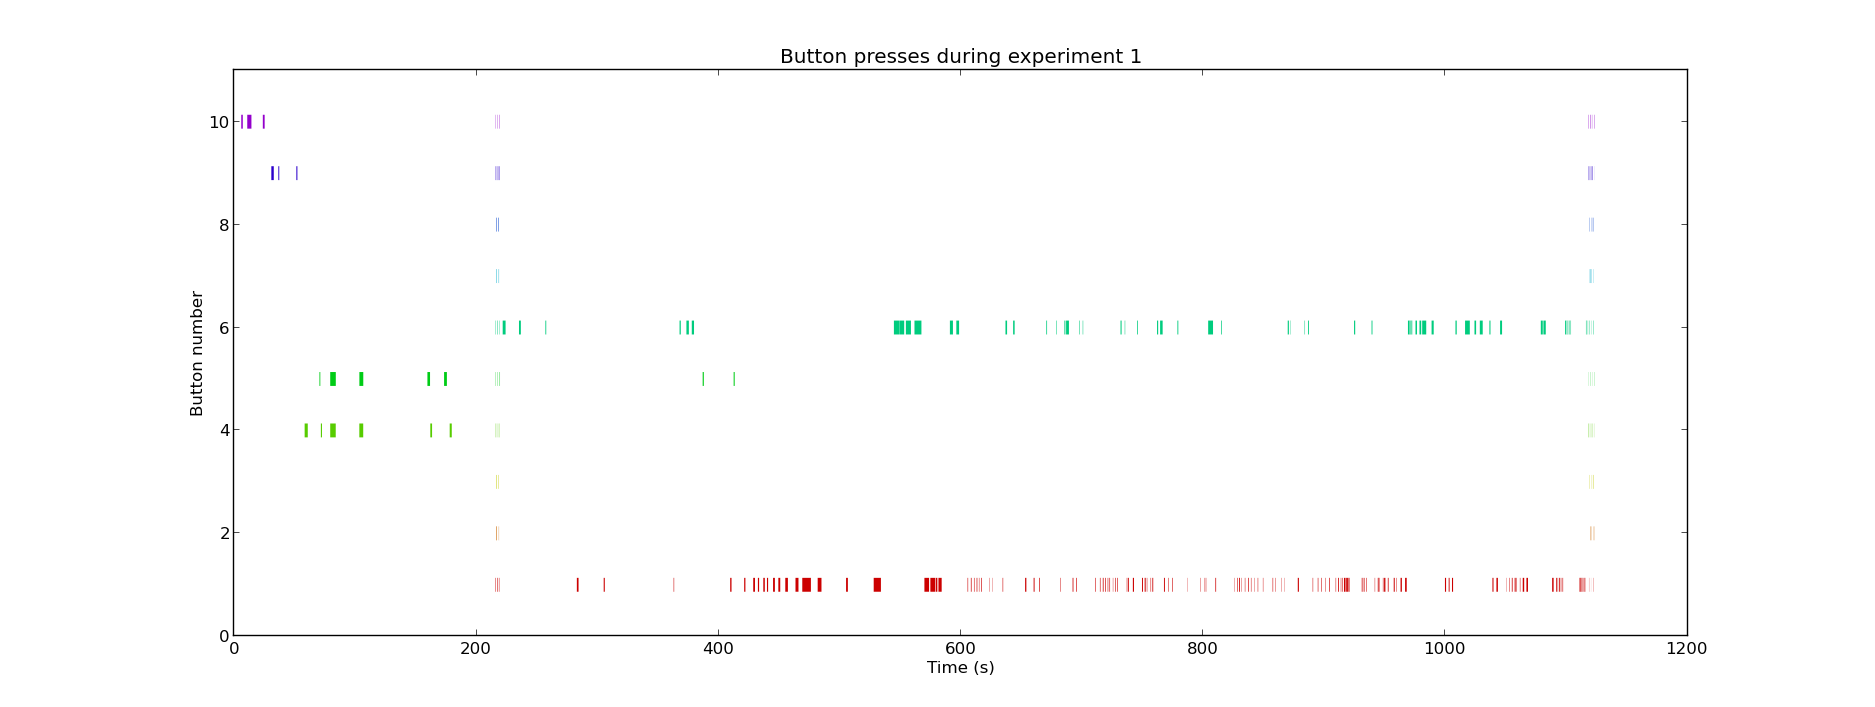
\includegraphics[width=\columnwidth]{timeline_experiment_1.png}
   		\caption{One full sequence of interaction, the events represent button press thought time and per channel. In this experiment the teacher, after trying several button, decided to send a ``reset'' signal by pressing all buttons. Then they successfully converged to a feedback based communication and are completing the task. At the end, the teacher signals the task is over by, once again, pressing all buttons.}
    \label{fig:timeline}
   	\end{center}
\end{figure}

Finally, figure~\ref{fig:understanding_per_feedback} is an attempt to describe what types of instruction where actually understood, misinterpreted, or ignored. While I still have to think and confirm the validity of this plot, it seems a good indication that positive and negative feedback, end, and reset are the most commonly understood instructions. 

\begin{figure}[H]
	\begin{center}
   		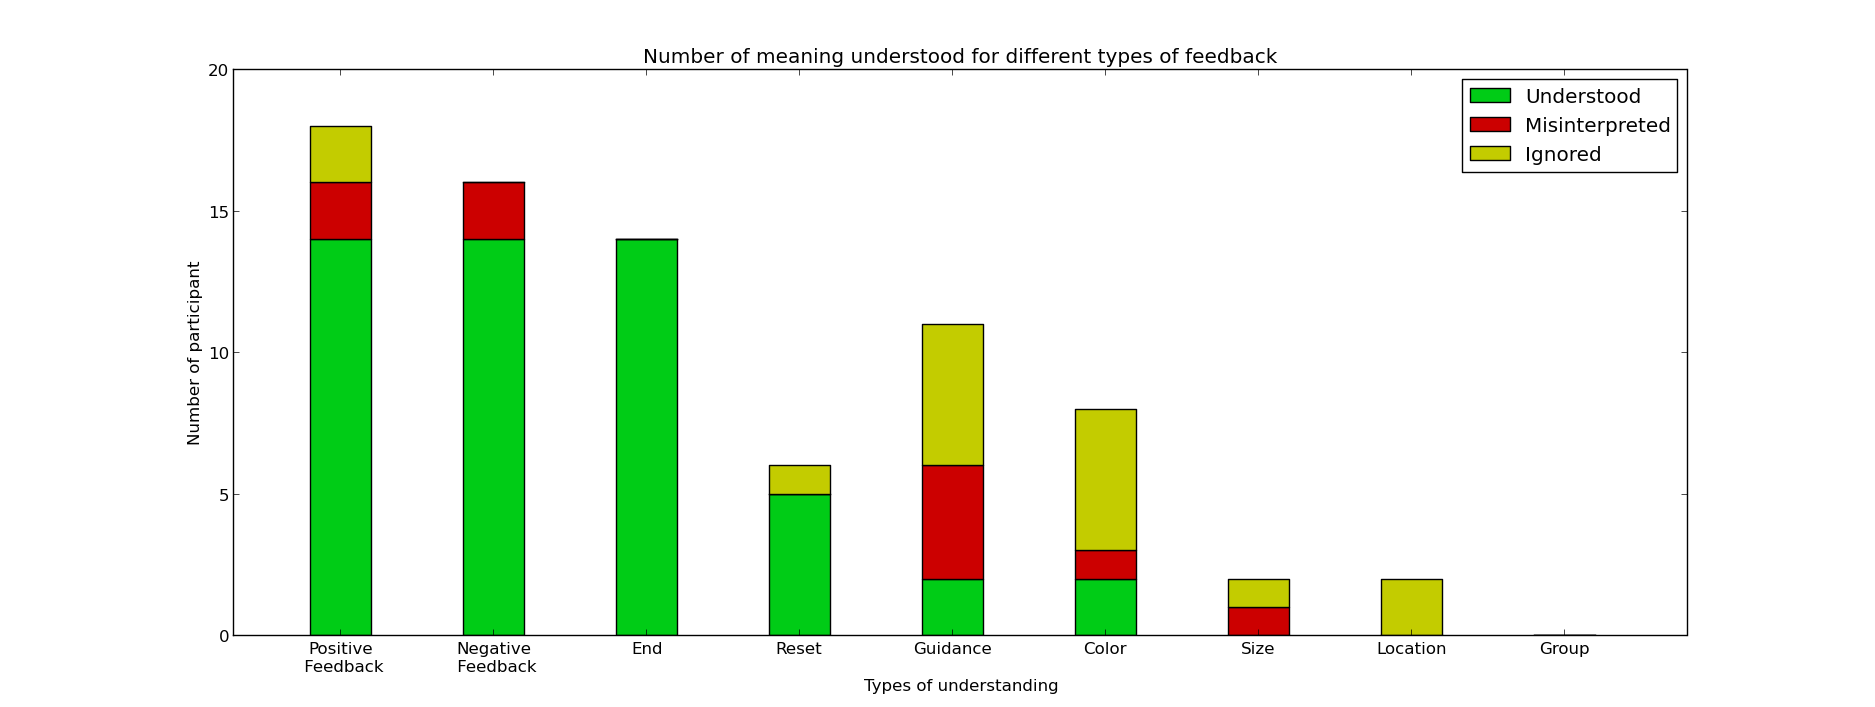
\includegraphics[width=\columnwidth]{understanding_per_feedback.png}
   		\caption{Learner type of understanding of different types of instruction from the teacher at the end of the experiment.}
    \label{fig:understanding_per_feedback}
   	\end{center}
\end{figure}

As a concluding remarks, I have also experienced some students affected by the so called confirmation bias. While interpreting negative feedback into positive they were going quite far in a wrong direction even if signal would seem contradictory for an outside observer. It was very difficult to re-assess their belief, they better thought the teacher was mistaking or were pursuing in a very improbable direction. I think no students were able to overcome the confirmation bias problem by themselves, leading either to a failed experiment or needed the teacher to produce a salient event to reset the experiment. With the recorded data, it is unfortunately not possible to quantify this phenomenon even if the figure~\ref{fig:feedback_switch_enhanced} gives a good first intuition.
